\documentclass[conference]{IEEEtran}
\IEEEoverridecommandlockouts
\usepackage{cite}
\usepackage{amsmath,amssymb,amsfonts}
\usepackage{algorithmic}
\usepackage{graphicx}
\usepackage{textcomp}
\usepackage{xcolor}
\def\BibTeX{{\rm B\kern-.05em{\sc i\kern-.025em b}\kern-.08em
    T\kern-.1667em\lower.7ex\hbox{E}\kern-.125emX}}
\begin{document}
\linespread{1.25}

\title{A Novel Wireless Sensor Network Based Rescue Management System}
\\
\\
\\
\\
\author{


\IEEEauthorblockN{KHUSHBU PAHWA}
\IEEEauthorblockA{\textit{Dept. of Electrical  Engineering} \\
\textit{Delhi Technological University}\\
Delhi, India \\
}
\and
\IEEEauthorblockN{ASHUTOSH BHARTI}
\IEEEauthorblockA{\textit{Dept. of Computer Engineering} \\
\textit{National Institute of Science and Technology}\\
Odisha, India \\
}
\and
\IEEEauthorblockN{KIRAN JYOTI SAHU}
\IEEEauthorblockA{\textit{Dept. of Computer Engineering} \\
\textit{National Institute of Science and Technology}\\
Odisha, India \\
}
}
\\
\\
\\
\maketitle

\begin{abstract}
In the aftermath of natural or man-made disasters, timely and efficient search and rescue operations play a crucial role in saving human lives. However, the overall effectiveness of such missions is often reduced due to the unavailability of real-time information about the location and condition of trapped or injured victims. The lack of communication infrastructure in disaster-hit regions further limits coordination between victims and rescue personnel.

This paper proposes a novel rescue management system based on Wireless Sensor Networks (WSN) and Internet of Things (IoT) technologies to address these challenges. The system integrates multiple sensors—such as temperature, humidity, pulse rate, accelerometer, and GPS—using NodeMCU-ESP8266 microcontrollers to collect real-time physiological and environmental data. The data is transmitted to a ThingSpeak cloud platform when network connectivity is available, and through an ad-hoc Wi-Fi mesh in offline mode. The model uses Received Signal Strength Indicator (RSSI)-based localization and employs an Artificial Neural Network (ANN) for distance estimation under varying environmental conditions \cite{b1}, \cite{b2}, \cite{b6}. The proposed framework is cost-effective, scalable, and adaptable for both connected and infrastructure-deficient environments, enabling faster victim detection and rescue response.
\end{abstract}


\begin{IEEEkeywords}
ANN, IoT, RSSI, Sensors, ThingSpeak Cloud, Wireless Sensor Network
\end{IEEEkeywords}
\section{Introduction}
Disaster management is a multidisciplinary challenge that involves rapid detection, communication, and coordination between various rescue agencies. In the critical “golden hour” after a disaster, timely access to accurate information about victims’ locations and physical conditions significantly improves survival rates. Unfortunately, during large-scale emergencies such as earthquakes, floods, or landslides, communication infrastructure often collapses, and traditional systems fail to provide the necessary situational awareness.

Wireless Sensor Networks (WSN) and IoT technologies offer a promising solution to bridge this information gap. WSNs enable the deployment of intelligent, interconnected sensor nodes capable of collecting, transmitting, and analyzing environmental and physiological data in real time \cite{b1}, \cite{b3}, \cite{b4}. These devices can operate independently or cooperatively to establish temporary communication networks, even in the absence of cellular coverage. Several studies have investigated the use of RSSI-based localization for indoor and outdoor tracking applications \cite{b1}, \cite{b2}, \cite{b6}. However, most prior work has not considered environmental variables such as temperature and humidity, which significantly influence signal propagation in outdoor environments \cite{b4}.


\section{Literature Review}
In \cite{b2}, authors used RSSI to measure the distance between two NodeMCUs and later applied curve-fitting to estimate the distance and percentage error. In \cite{b3}, DHT11 sensor was used with Arduino to send data to ThingSpeak. In \cite{b4}, the impact of temperature and humidity on RSSI was studied — temperature had a high negative influence on signal strength. This motivated us to build a robust RSSI-based localisation system incorporating temperature and humidity. The negative correlation between temperature and RSSI suggests that as temperature increases, the signal strength tends to degrade, possibly due to the physical properties of the medium through which the signal travels. Humidity, on the other hand, may cause scattering or absorption of the radio waves, further influencing the received signal strength. To account for these environmental factors, a robust localization system must integrate real-time measurements of both temperature and humidity alongside traditional RSSI values.

By incorporating these variables into the localization algorithm, we aim to mitigate the inaccuracies caused by fluctuating environmental conditions. This could lead to more precise positioning, especially in dynamic environments like outdoor settings or industrial areas.



In \cite{b5}, TOA and TDOA techniques were compared and it was found that RSSI-based localisation is hardware-efficient. In \cite{b6}, polynomial approximation and Neural Networks were used to relate RSSI and distance but without accounting for environmental factors.

\section{Rescue Management System Model}

\subsection{Requirements of Rescue Personnel}
\begin{itemize}
    \item Rescue personnel need location-based survey data to identify where more human lives may exist.
    \item Feedback from victims about their condition aids in timely rescue.
    \item Intelligent devices can alert rescue teams even if victims are unconscious.
    \item In case of infrastructure damage, ad-hoc networks should be deployable on-site.
\end{itemize}

\subsection{Requirements of Victims}
\begin{itemize}
    \item Victims should be able to inform rescue personnel via mobile device.
    \item If unconscious or unable to communicate, devices should send distress signals automatically.
    \item Data should propagate through ad-hoc NodeMCU networks when GSM fails.
\end{itemize}

\section{Working Methodology}

\subsection{Data Collection from Sensors}
The device for victims consists of NODEMCU-ESP8266 integrated with DHT-11, pulse sensor, and MPU6050 accelerometer and gyroscope. The rescuer carries a similar setup. The total cost per unit is approximately ₹1500.
\subsection{Data Transfer}
When a network is available, data is transferred to ThingSpeak server \cite{b8}. In offline mode, data is exchanged between nearby NodeMCUs over Wi-Fi. Two SSIDs are created—one for hotspot (ad-hoc) and another for cloud upload. Arduino IDE is used for coding both modes.


\begin{figure}[htbp]
\centering
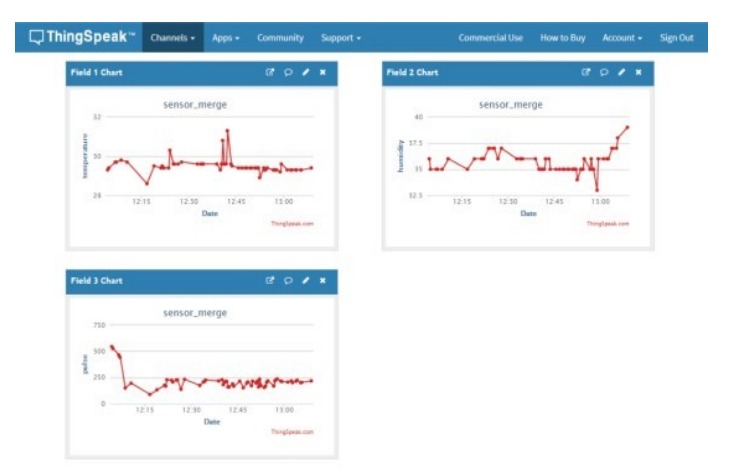
\includegraphics[width=0.45\textwidth]{figure1.jpg} % Replace with your actual image filename
\caption{Data transfer architecture showing online and offline communication paths between NodeMCU nodes and ThingSpeak cloud.}
\label{fig:data_transfer}
\end{figure}

\subsection{Collection of RSSI values}

In \cite{ref2}, the authors used mean of 300 RSSI values at each known distance, as a measure for distance estimation in indoor environment. To ensure the robustness of our approach, we measured the RSSI values in the outdoor conditions taking into account the temperature and humidity values. The data was obtained by using a DHT-11 temperature and humidity sensor interfaced with a NodeMCU node which acted as the receiver node and the other NodeMCU was placed apart at distances from 1 to 42 meters, and 100 RSSI values were obtained for each distance and transferred to PLXDAP software \cite{ref9} using the COM port. The dataset was generated over a period of 15 days at three times of the day in morning, afternoon and evening for carrying out a comprehensive analysis consisting of varied environmental conditions. Table~\ref{tab:rssi} shows a sample set of RSSI values obtained for different temperature and humidity at distances from 1 to 10 meters. The table validates the variation in RSSI values due to environmental conditions. The table shows average RSSI values obtained for two sets of temperature and humidity.

\renewcommand{\arraystretch}{1.3} % Increase row height by 30%
\begin{table}[h!]
\centering
\caption{RSSI values in outdoor conditions}
\label{tab:rssi}
\resizebox{\columnwidth}{!}{%
\begin{tabular}{|c|c|c|c|c|c|c|}
\hline
\textbf{Distance (m)} & \textbf{Temp 1 (°C)} & \textbf{Hum. 1 (\%)} & \textbf{RSSI 1 (dBm)} & \textbf{Temp 2 (°C)} & \textbf{Hum. 2 (\%)} & \textbf{RSSI 2 (dBm)} \\ \hline
1  & 26 & 63 & -63.30 & 33 & 49 & -71.74 \\ \hline
2  & 26 & 81 & -73.29 & 33 & 47 & -76.12 \\ \hline
3  & 26 & 79 & -79.54 & 34 & 47 & -81.32 \\ \hline
4  & 26 & 82 & -83.94 & 34 & 44 & -82.69 \\ \hline
5  & 26 & 82 & -84.17 & 34 & 44 & -86.92 \\ \hline
6  & 26 & 80 & -85.80 & 35 & 43 & -87.12 \\ \hline
7  & 26 & 80 & -86.04 & 35 & 43 & -88.70 \\ \hline
8  & 26 & 81 & -88.12 & 36 & 42 & -89.21 \\ \hline
9  & 26 & 82 & -89.35 & 36 & 42 & -90.12 \\ \hline
10 & 26 & 78 & -89.47 & 33 & 51 & -90.30 \\ \hline
\end{tabular}%
}
\end{table}


\section{Training the Network}
A dataset of 1000 readings was prepared with distance as the label and temperature, humidity, and RSSI as features. MATLAB Neural Network Toolbox \cite{b10} was used for training. Data was normalized using Min-Max normalization. The neural network consisted of one hidden layer with \textit{tansig} activation:
\begin{equation}
tansig(x) = \frac{2}{1 + e^{-2x}} - 1
\end{equation}
The output layer used a linear activation function.

\section{Performance Analysis}
The neural network model achieved the following:
\begin{table}[htbp]
\caption{Model Accuracy and Mean Square Error (MSE) Results}
\centering
\begin{tabular}{|c|c|}
\hline
\textbf{Training accuracy} & mean square error: 0.057 \\
\hline
\textbf{Testing accuracy} & mean square error:  0.108 \\
\hline
\textbf{Validation accuracy} & mean square error:  0.090 \\
\hline
\end{tabular}
\label{tab:accuracy}
\end{table}

\section{Conclusion and Future Work}
A low-cost robust setup for disaster victim localisation in both online and offline modes was developed. Environmental factors such as temperature and humidity were considered for distance estimation. RSSI can help locate victims where GPS fails due to infrastructure damage. Future work includes integrating direction detection and further optimizing outdoor localization.

\section*{Acknowledgment}
The authors express gratitude to Prof. Siba Kumar Udgata, School of Computer and Information Sciences, University of Hyderabad, for his guidance and valuable insights during this research.

\bibliographystyle{IEEEtran}
\bibliography{references}


\end{document}
